\documentclass[12pt]{article}

\usepackage[utf8]{inputenc}
\usepackage{latexsym,amsfonts,amssymb,amsthm,amsmath,graphicx}
\usepackage[parfill]{parskip}

\DeclareMathAlphabet{\mymathbb}{U}{BOONDOX-ds}{m}{n}

\setlength{\parindent}{0in}
\setlength{\oddsidemargin}{0in}
\setlength{\textwidth}{6.5in}
\setlength{\textheight}{8.8in}
\setlength{\topmargin}{0in}
\setlength{\headheight}{18pt}

\newcommand{\xb}{\mathbf{x}}
\newcommand{\yb}{\mathbf{y}}
\newcommand{\ab}{\mathbf{a}}
\newcommand{\abi}{\ab_i}
\newcommand{\xnorm}{\lVert \mathbf{\xb} \rVert}
\newcommand{\sumin}{\sum_{i = 1}^n}
\newcommand{\ellsh}{\ell_{sh}}
\newcommand{\ax}{\abi^T\xb}
\newcommand{\atilde}{\mathbf{\tilde{A}}}
\newcommand{\id}{\mathbf{I}}
\newcommand{\ones}{\mathbf{1}}

\title{EE-556 Homework 1}
\author{Edoardo Debenedetti}

\begin{document}

\maketitle

\vspace{0.5in}



\section*{Problem 1 - Geometric properties of the objective function $f$}

Assuming $\mu = 0$, the smooth Hinge loss function $f$ becomes:

\begin{equation} \label{def:hinge_loss}
    f(x) = \ellsh(\xb) + \frac{\lambda}{2} \xnorm ^ 2
\end{equation}

where

\begin{equation} \label{def:l}
    \ellsh = \frac{1}{n} \sumin g_i(\xb)
\end{equation}

and

\begin{equation}
    g_i(\xb) = \begin{cases} \label{def:g}
    \frac{1}{2} - b_i(\ax)         & b_i(\ax) < 0 \\
    \frac{1}{2}(1 - b_i(\ax))^2    & 0 \leq b_i(\ax) \leq 1 \\
    0                                   & 1 \le b_i(\ax)
\end{cases}
\end{equation}

\subsection*{(a) Gradient of $f$}

\subsection*{Computation of the gradient}

\begin{proof}
Since the gradient is a linear operator:

\begin{equation}
    \nabla f(\xb) = \nabla \ellsh + \nabla \frac{\lambda}{2} \xnorm ^ 2
\end{equation}

We can first compute $\nabla \frac{\lambda}{2} \xnorm$:

\begin{gather}
    \nabla \frac{\lambda}{2} \xnorm ^ 2 =
    \frac{\lambda}{2} \nabla \xnorm ^ 2 =
    \frac{\lambda}{2} \nabla \sumin |x_i|^2 = \nonumber
    \frac{\lambda}{2} \sumin \nabla x_i^2 = \\
     = \frac{\lambda}{2}2\xb =
    \lambda \xb \label{eq:grad_lambda}
\end{gather}

Now, let us compute $\nabla \ellsh$:

\begin{equation}
    \nabla \ellsh = \nabla \frac{1}{n} \sumin g_i(\xb) = \frac{1}{n} \sumin \nabla g_i(\xb)
\end{equation}

Where $\nabla g_i(\xb)$ is the gradient of \eqref{def:g}

\begin{equation}
    \nabla g_i(\xb) = \begin{cases}
        \nabla \left [\frac{1}{2} - b_i(\ax)\right]         & b_i(\ax) < 0 \\
        \nabla \left [\frac{1}{2}(1 - b_i(\ax))^2\right]    & 0 \leq b_i(\ax) \leq 1 \\
        \nabla 0                                            & 1 \le b_i(\ax)
    \end{cases}
\end{equation}

The case where $1 \le b_i(\ax)$ is trivial, since
\begin{equation} \label{eq:grad_0_case}
    \nabla 0 = 0
\end{equation}

In the case where $b_i(\ax) < 0$:

\begin{equation} \label{eq:grad_linear_case}
    \nabla \left [\frac{1}{2} - b_i(\ax)\right] = \nabla (-b_i(\ax)) = -b_i\abi
\end{equation}

Next, in the case where $0 \leq b_i(\ax) \leq 1$:

\begin{gather}
    \nabla \left [\frac{1}{2}(1 - b_i(\ax))^2\right] = \nonumber
    -\frac{1}{2} 2 b_i\abi(1 - b_i(\ax)) = \\ \label{eq:grad_quadr_case}
    -b_i\abi(1 - b_i(\ax)) = b_i\abi(b_i(\ax) - 1)
\end{gather}

Finally, combining \eqref{eq:grad_0_case}, \eqref{eq:grad_linear_case} and \eqref{eq:grad_quadr_case}, we get:
\begin{equation}
    \nabla g_i(\xb) = \begin{cases}
            -b_i\abi                & b_i(\ax) < 0 \\
            b_i\abi(b_i(\ax) - 1)   & 0 \leq b_i(\ax) \leq 1 \\
            0                       & 1 \le b_i(\ax)
    \end{cases}
\end{equation}

Now, let us define, as in the problem statement, $\atilde:=[b_1\ab_1, ..., b_n\ab_n]^T$, and $\id_L, \id_Q$ as the diagonal $n \times n$ matrices such that $\id_L(i,i) = 1$ if $b_i(\ax) < 0$ and $\id_Q(i,i) = 1$ if $0 \leq b_i(\ax) \leq 1$, and $0$ otherwise.

We can observe that $\atilde^T\id$ is the matrix whose $i$-th column is $b_i\abi$. Instead, $\atilde^T\id_L$'s $i$-th columns will be non-zero only in the case where $b_i(\ax) < 0$. Then it is possible to represent this case of $\nabla g_i(\xb)$ where $b_i(\ax) < 0$ as

\begin{equation} \label{eq:grad_matrix_linear_case}
    -\frac{1}{n}\atilde^T\id_L\ones
\end{equation}

since multiplying $\atilde^T\id_L$ by $\ones$ will give as result the vector containing the sum of the elements of each column, which means the element-wise sum of the different $j$-th components of the $i$-th gradients relative to each $g_i(\xb)$. Each $j$-th component can be written as

\begin{equation*}
    \sum_{i \ \in \ \{i \ | \ b_i(\ax) \ < \ 0\}}^{n} a_{i,j} b_j
\end{equation*}

In a similar fashion, $\atilde^T\id_Q$ is the matrix whose $i$-th column is $\abi b_i$ only if $i$ is such that $0 \leq b_i(\ax) \leq 1$. Moreover, $\atilde \xb$ is the vector such that $[\atilde \xb]_n = \sumin b_i\abi\xb$. Consequently, $\atilde\id_Q[\atilde \xb - \ones]$ is the vector whose $j$-th component is

\begin{equation*}
    [\atilde^T\id_Q[\atilde \xb - \ones]]_j =
    \sum_{i \ \in \ \{i \ | \ 0 \ \leq \ b_i(\ax) \ \leq \ 1\}}^{n} b_j a_{i, j} (b_j(\ax) - 1)
\end{equation*}

if $0 \leq b_i(\ax) \leq 1$. Then, with 

\begin{equation} \label{eq:grad_matrix_quadratic_case}
    \frac{1}{n}\atilde^T\id_Q[\atilde \xb - \ones]
\end{equation}

we can represent the components of $\nabla g_i(\xb)$ in the aforementioned case.

Combining \eqref{eq:grad_matrix_linear_case} and \eqref{eq:grad_matrix_quadratic_case}, it is proven that

\begin{equation} \label{eq:grad_l_sh}
    \nabla \ellsh = \frac{1}{n}(\atilde^T\id_Q[\atilde \xb - \ones] - \atilde^T\id_L\ones)
\end{equation}

Finally, combining \eqref{eq:grad_lambda} and \eqref{eq:grad_l_sh} we get the final result

\begin{equation}
    \nabla f(\xb) = \lambda\xb + \frac{1}{n}\atilde^T\id_Q[\atilde \xb - \ones] - \frac{1}{n}\atilde^T\id_L\ones
\end{equation}

\end{proof}

\subsection*{L-Lipschitz continuity of the gradient}

\begin{proof}
By definition, a function $f$ has L-Lipschitz continuous gradient if $\exists L < \infty$ such that:
\begin{equation} \label{eq:l-smooth}
    \lVert \nabla f(\xb) - \nabla f(\yb) \rVert \leq L \lVert \xb - \yb \rVert
\end{equation}

So, let us compute the left term of the inequality for our objective function $f$:

\begin{gather}
    \lVert \nabla f(\xb) - \nabla f(\yb) \rVert = \nonumber \\
    \left \lVert \lambda\xb + \frac{1}{n}\atilde^T\id_Q[\atilde \xb - \ones] - \frac{1}{n}\atilde^T\id_L\ones - \left ( \lambda\yb + \frac{1}{n}\atilde^T\id_Q[\atilde \yb - \ones] - \frac{1}{n}\atilde^T\id_L\ones \right ) \right \rVert \label{eq:first-l}
\end{gather}

We can then observe that the linear parts cancel, that we can take out lambda and expand the expressions in the quadratic region. Eq. \ref{eq:first-l} becomes:

\begin{equation} \label{eq:second-l}
        \left \lVert \lambda (\xb - \yb) + \frac{1}{n}\atilde^T\id_Q\atilde\xb - \frac{1}{n}\atilde^T\id_Q\atilde\yb - \frac{1}{n}\atilde^T\id_Q + \frac{1}{n}\atilde^T\id_Q \right\rVert 
\end{equation}

Again, we can cancel the last two factors, and take out the factor $\frac{1}{n}\atilde^T\id_Q\atilde$. We can also note that since we are now dealing only with elements in the quadratic region and there is no contribution from elements in the linear region, we can consider $\id_Q$ as $\mathbb{I}$ and then we can cancel it. As a consequence, eq. \ref{eq:second-l} becomes:

\begin{gather}
    \left \lVert \lambda(\xb - \yb) + \frac{1}{n}\atilde^T\atilde (\xb - \yb) \right \rVert = \nonumber \\
    \left \lVert \left ( \lambda + \frac{1}{n}\atilde^T\atilde \right ) (\xb - \yb) \right \rVert \label{eq:third-l}
\end{gather}

We can now use Cauchy-Schwartz and triangle inequalities:

\begin{gather}
    \left \lVert \left ( \lambda + \frac{1}{n}\atilde^T\atilde \right ) (\xb - \yb) \right \rVert \leq
    \left \lVert \lambda + \frac{1}{n}\atilde^T\atilde \right \rVert \left \lVert \xb - \yb \right \rVert \leq \nonumber \\
    \leq \left ( \lVert \lambda \rVert + \left \lVert \frac{1}{n}\atilde^T\atilde \right \rVert \right ) \left \lVert \xb - \yb \right \rVert = \nonumber \\
    \left (\lambda + \frac{1}{n} \lVert \atilde^T \rVert \lVert \atilde \rVert  \right ) \left \lVert \xb - \yb \right \rVert \label{eq:fourth-l}
\end{gather}

Since $\lambda$ is a scalar, its norm is the number itself. Moreover, since $\frac{1}{n}$ is a scalar as well, we can take it out of the norm. We can now combine equations \ref{eq:l-smooth}, \ref{eq:third-l} and \ref{eq:fourth-l} and get the following result:

\begin{equation}
    \left ( \lambda + \frac{1}{n} \lVert \atilde^T \rVert \lVert \atilde \rVert \right ) \left \lVert \xb - \yb \right \rVert \leq L \lVert \xb - \yb \rVert
\end{equation}

if $L = \lambda + \frac{1}{n} \lVert \atilde^T \rVert \lVert \atilde \rVert$. Finally, recalling that $\atilde:=[b_1\ab_1, ..., b_n\ab_n]^T$ where $b_n \in \{-1, 1\}$, we can note that $\lVert \atilde \rVert = \lVert \mathbf{A} \rVert$, since the norm is computed taking in account the absolute value of each entry of a matrix. Hence, as a final result,

\begin{equation}
    f(\xb) \in \mathcal{F}_{L}^{1, 1}
\end{equation}

with $L = \lambda + \frac{1}{n} \lVert \mathbf{A}^T \rVert \lVert \mathbf{A} \rVert$.


\end{proof}

\subsection*{(b) Hessian of $f$}
\begin{proof}
Assuming that $\id_L = \mathbb{I}$, we can deduce that $\id_L = \mymathbb{0}$, since it would mean that $\forall i \in [1,\ n], \ b_i(\abi^T\xb) \ < \ 0$. Then some simple computations can show that

\begin{equation}
    \nabla f(\xb) = \lambda \xb + \frac{1}{n} \atilde^T(\atilde\xb) - \atilde^T
\end{equation}

We can then compute the Hessian $\nabla^2 f(\xb)$ as $\nabla \cdot \nabla f(\xb)$, that is

\begin{gather}
    \nabla^2 f(\xb) = \nabla \cdot \nabla f(\xb) = \nabla \cdot \lambda \xb + \nabla \cdot \left [ \frac{1}{n} \atilde^T(\atilde\xb) - \atilde^T \right ] \nonumber = \\
    = \lambda \nabla \cdot \xb + \frac{1}{n} \atilde^T (\atilde \nabla \cdot \xb) = \nonumber \\
    = \lambda \mathbb{I} + \frac{1}{n} \atilde^T \atilde
\end{gather}

Hence, $\nabla^2 f(\xb) = \lambda \mathbb{I} + \frac{1}{n} \atilde^T \atilde$. Moreover, $f(\xb)$ is twice differentiable because $\nabla ^2 f(\xb)$ is continuous over $\mathbb{R}^p$

\end{proof}

\subsection*{(c) Strong convexity of $f$}
\begin{proof}
First, let use recall that $f(\xb) = \ellsh(\xb) + \frac{\lambda}{2} \xnorm^2$ and that a function $f(\xb)$ is $\mu$-strongly convex iff, given $h(\xb) = f(\xb) - \frac{\mu}{2} \xnorm^2$, $h(\xb)$ is convex. In the case of the smooth Hinge loss function,

\begin{equation}
    h(\xb) = \ellsh + \frac{\lambda}{2} \xnorm^2 - \frac{\mu}{2} \xnorm^2
\end{equation}

Now, setting $\mu = \lambda$, we get that $h(\xb) = \ellsh(x)$. We know that $\ellsh$ is convex, and then $h(\xb)$ us convex as well. Thus,

\begin{equation}
    f(\xb) \in \mathcal{F}_{L, \mu}^{2, 1}
\end{equation}

with $L = \lambda + \frac{1}{n} \lVert \mathbf{A}^T \rVert \lVert \mathbf{A} \rVert$ and $\mu = \lambda$.

\end{proof}

\section*{First order methods for linear SVM}

\begin{figure}[h]
    \centering
    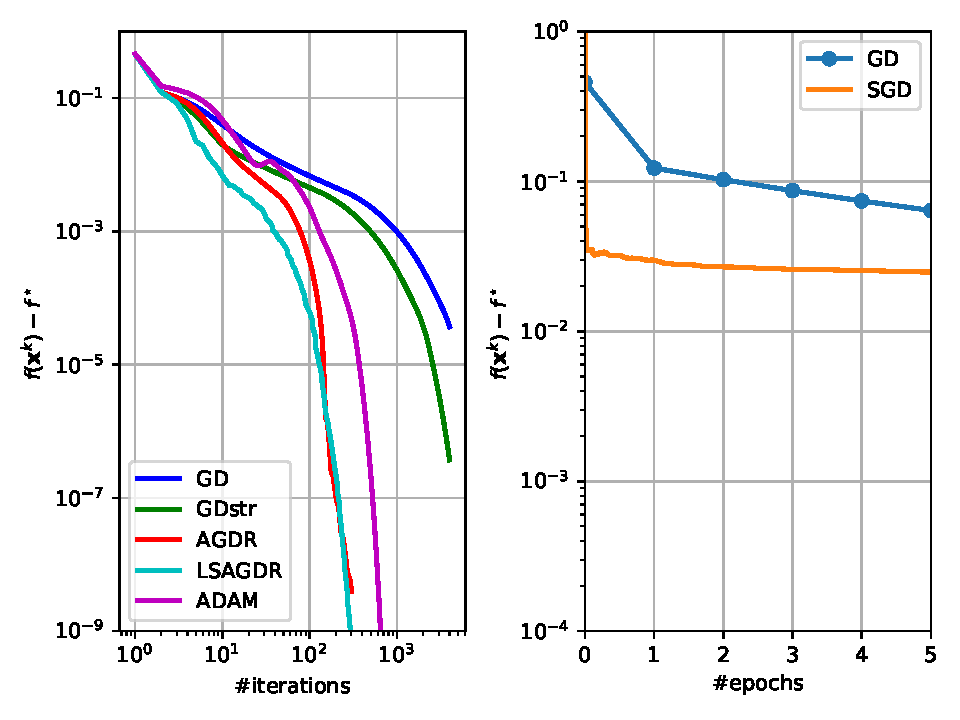
\includegraphics[width=10cm]{hw1/codes/fig_ex1.pdf}
    \caption{Caption}
    \label{fig:my_label}
\end{figure}

\end{document}